\documentclass{article}

\usepackage{graphicx}
\usepackage{tikz}
\usepackage{tikzsymbols}
\usetikzlibrary{calc,patterns,shapes.geometric}
\pagestyle{empty}
\usepackage[margin=0pt]{geometry}
\geometry{papersize={14in,12in}}

\def\centerarc[#1](#2)(#3:#4:#5){\draw[#1] ($(#2)+({#5*cos(#3)},{#5*sin(#3)})$) arc (#3:#4:#5);}

\begin{document}
	\begin{figure}
		\centering
		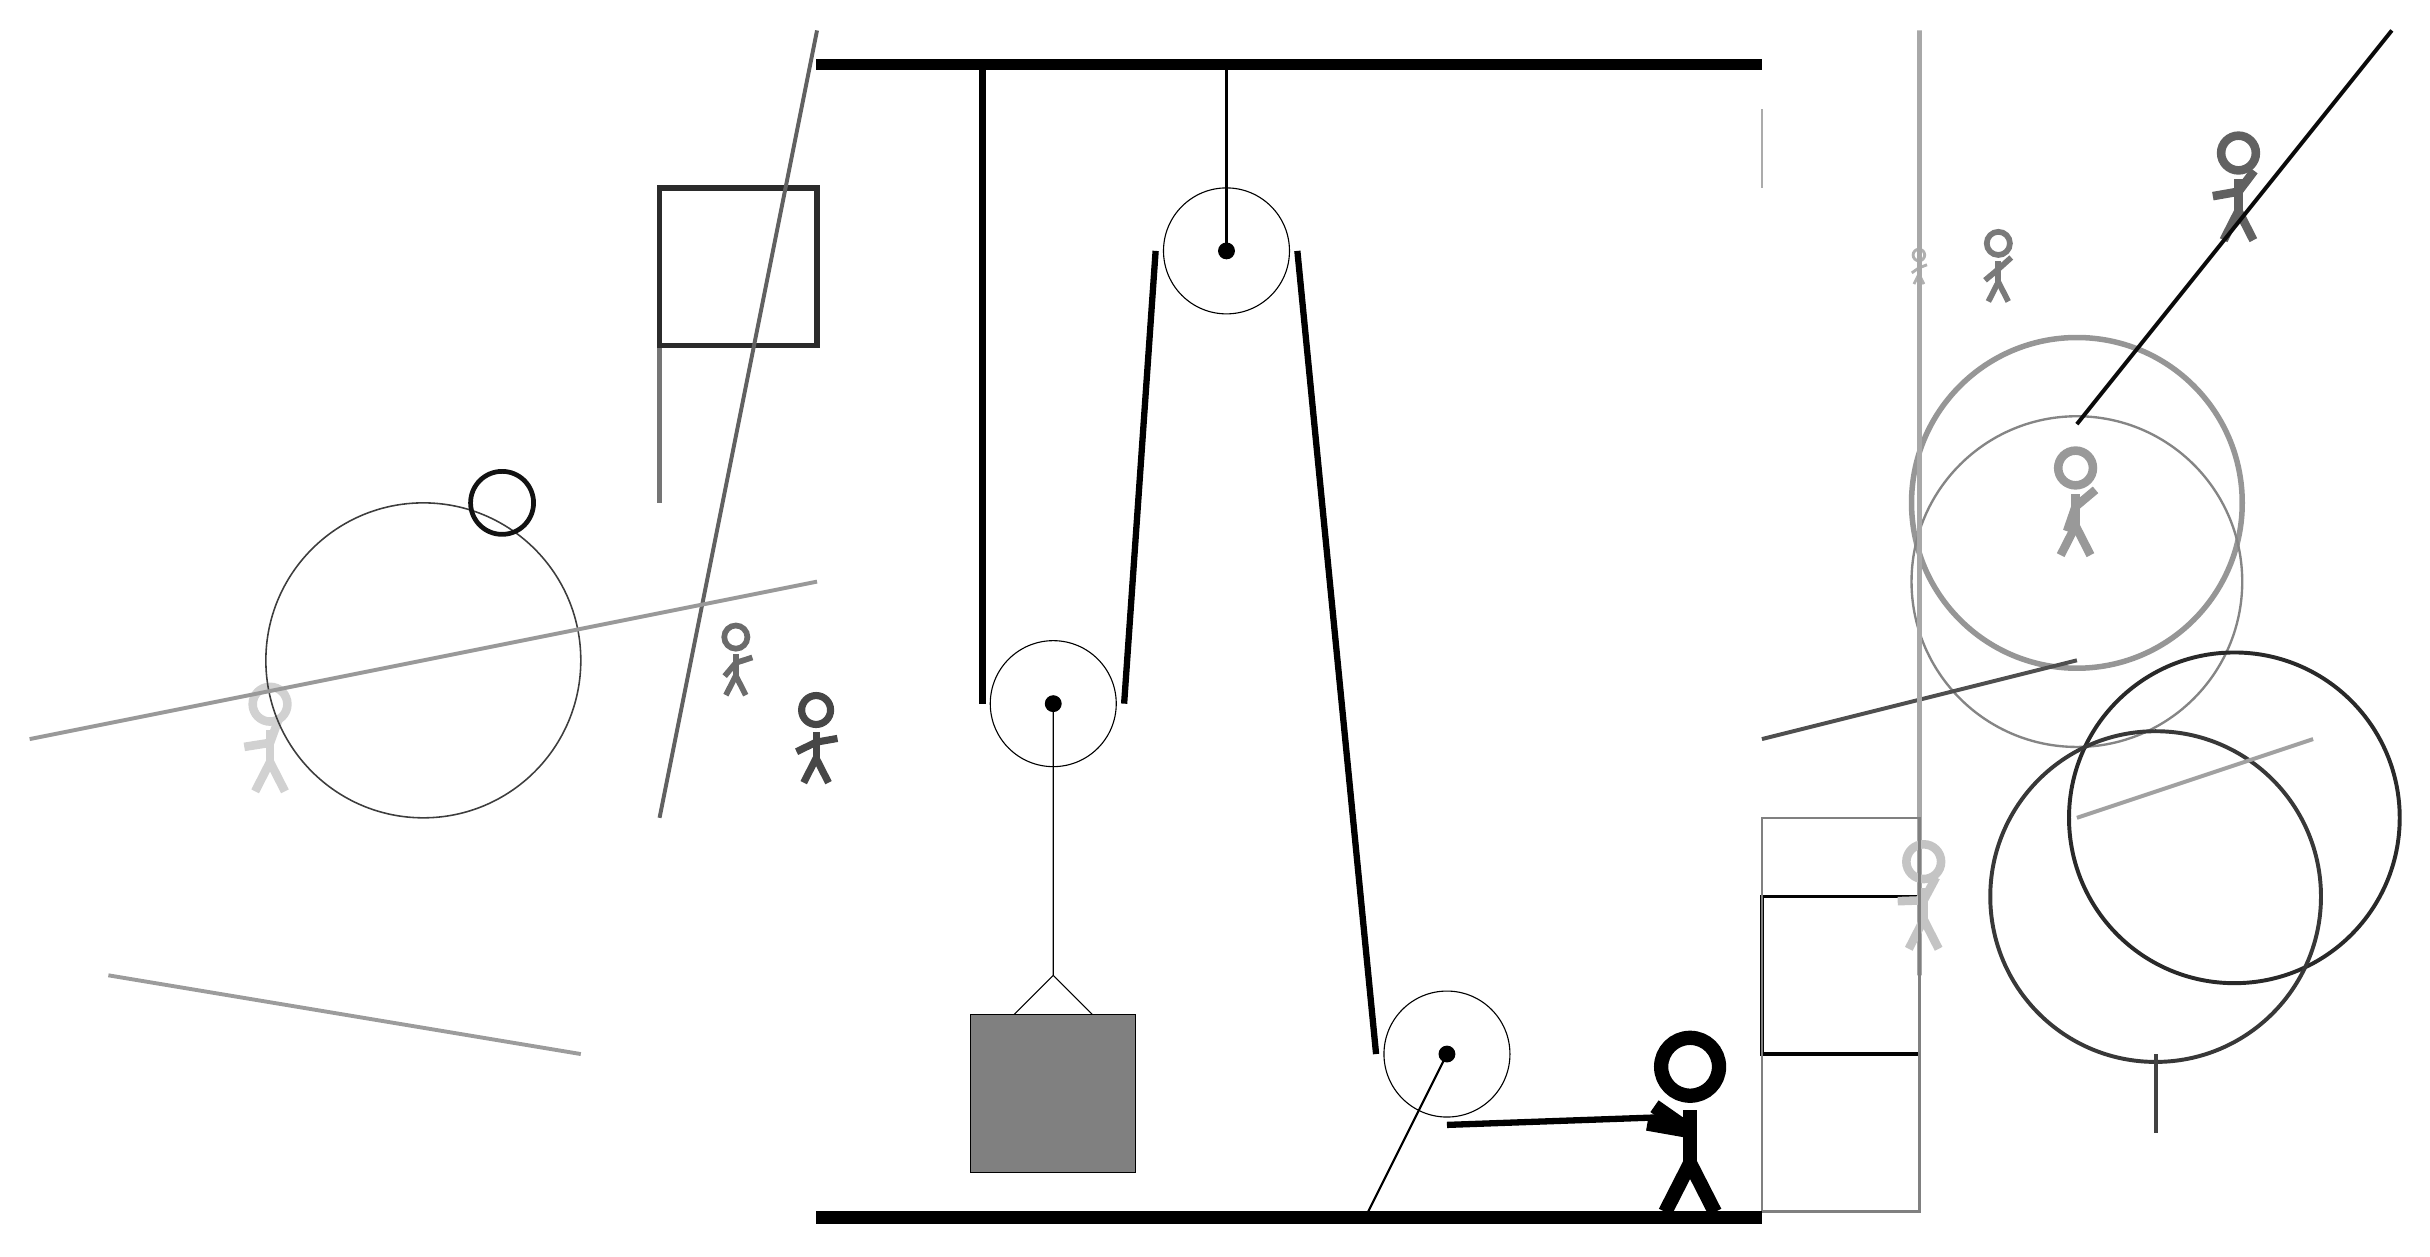
\begin{tikzpicture}
			%%%%% START %%%%%
			
			\draw[fill=black] (-2, 11.5) rectangle (10, 11.625);
			
			\draw (3.2, 9.2) circle (0.8);
			\draw[fill=black] (3.2, 9.2) circle (0.1);
			\draw[thick] (3.2, 9.2) -- (3.2, 11.5);
			
			\draw (6, -1) circle (0.8);
			\draw[fill=black] (6, -1) circle (0.1);
			\draw[thick] (6, -1) -- (5, -3);
			
			\draw (1, 3.45) circle (0.8);
			\draw[fill=black] (1, 3.45) circle (0.1);
			
			\draw (1, 3.45) -- (1, 0.0) -- (0.5, -0.5);
			\draw (1, 0.0) -- (1.5, -0.5);
			\draw[fill=black!50] (-0.05, -0.5) rectangle (2.05, -2.5);
			
			\draw[line width=0.8mm] (0.1, 11.5) -- (0.1, 3.45);
			\centerarc[line width=0.8mm](1, 3.45)(180:360:0.9);
			\draw[line width=0.8mm](1.9, 3.45) -- (2.3, 9.2);
			\centerarc[line width=0.8mm](3.2, 9.2)(0:180:0.9);
			\draw[line width=0.8mm](4.1, 9.2) -- (5.1, -1);
			\centerarc[line width=0.8mm](6, -1)(180:270:0.9);
			\draw[line width=0.8mm](6, -1.9) -- (8.8, -1.8);
			
			\node[line width=0.7mm, color=black!58] at (-3, 4) {\Strichmaxerl[4][50][18]};
			
			\draw [line width=0.7mm, color=black!41](14, 6) circle (2.1);
			\draw[line width=0.4mm, color=black!99] (12, -1) rectangle (10, 1);
			\draw[line width=0.2mm, color=black!33] (10, 10) rectangle (10, 11);
			\node[line width=0.2mm, color=black!52] at (13, 9) {\Strichmaxerl[4][40][42]};
			\draw [line width=0.3mm, color=black!48](14, 5) circle (2.1);
			
			\node[line width=0.2mm, color=black!72] at (-2, 3) {\Strichmaxerl[5][26][10]};
			\draw[line width=0.5mm, color=black!39](-5, -1) -- (-11, 0);
			\node[line width=0.5mm, color=black!31] at (12, 9) {\Strichmaxerl[2][35][21]};
			
			\node[line width=0.6mm, color=black!18] at (-9, 3) {\Strichmaxerl[6][9][70]};
			\draw [line width=0.5mm, color=black!84](16, 2) circle (2.1);
			\draw [line width=0.2mm, color=black!76](-7, 4) circle (2.0);
			\draw[line width=0.5mm, color=black!69](14, 4) -- (10, 3);
			\draw [line width=0.5mm, color=black!78](15, 1) circle (2.1);
			\draw[line width=0.5mm, color=black!37](14, 2) -- (17, 3);
			\node[line width=0.6mm, color=black!62] at (16, 10) {\Strichmaxerl[6][10][53]};
			\draw[line width=0.6mm, color=black!54] (-4, 8) rectangle (-4, 6);
			\draw[line width=0.7mm, color=black!34] (12, 0) rectangle (12, 12);
			\draw[line width=0.5mm, color=black!96](14, 7) -- (18, 12);
			\draw[line width=0.7mm, color=black!83] (-2, 10) rectangle (-4, 8);
			\draw[line width=0.5mm, color=black!62](-4, 2) -- (-2, 12);
			
			\node[line width=0.4mm, color=black!23] at (12, 1) {\Strichmaxerl[6][2][62]};
			\draw[line width=0.5mm, color=black!40](-2, 5) -- (-12, 3);
			\node[line width=0.7mm, color=black!40] at (14, 6) {\Strichmaxerl[6][71][40]};
			\draw [line width=0.6mm, color=black!93](-6, 6) circle (0.4);
			
			\draw[line width=0.5mm, color=black!74](15, -2) -- (15, -1);
			
			\draw[line width=0.3mm, color=black!50] (12, -3) rectangle (10, 2);
			
			\node at (9, -1.9) {\Strichmaxerl[10][-35][170]};
			
			\draw[fill=black] (-2, -3) rectangle (10, -3.15);
			
			%%%%% END %%%%%
		\end{tikzpicture}
	\end{figure}	
\end{document}